% Name: Normal distribution
% Description: The standard normal density with the area within one standard deviation of the mean shaded and the 68% that it holds marked.
% Tags: normal distribution, Gaussian, standard deviation, probability density

\usepackage{pgfplots}
\usepgfplotslibrary{fillbetween}
\pgfplotsset{compat=1.18}

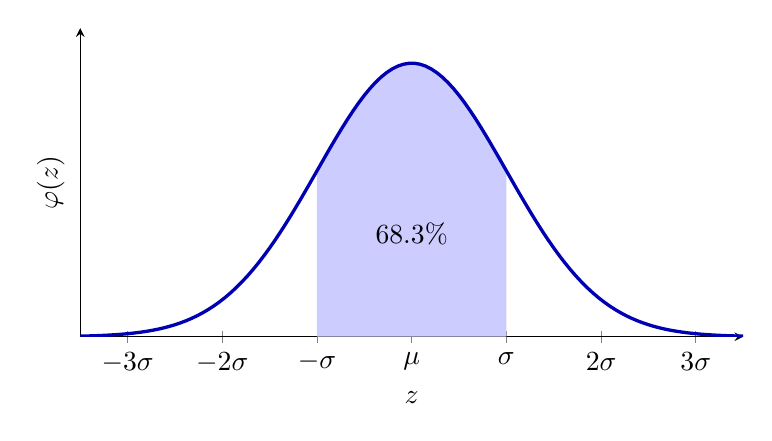
\begin{tikzpicture}
  \begin{axis}[
    width=10cm, height=5.5cm, domain=-3.5:3.5, samples=120,
    axis lines=left, xlabel=$z$, ylabel={$\varphi(z)$},
    xtick={-3,-2,-1,0,1,2,3}, xticklabels={$-3\sigma$,$-2\sigma$,$-\sigma$,$\mu$,$\sigma$,$2\sigma$,$3\sigma$},
    ymin=0, ymax=0.45, ytick=\empty, enlarge x limits=false,
  ]
    \addplot[name path=curve, very thick, blue!70!black] {exp(-x^2/2)/sqrt(2*pi)};
    \path[name path=floor] (axis cs:-3.5,0) -- (axis cs:3.5,0);
    \addplot[blue!20] fill between[of=curve and floor, soft clip={domain=-1:1}];
    \node at (axis cs:0,0.15) {68.3\%};
  \end{axis}
\end{tikzpicture}
